\section{Expressing Computation with Closures}\label{concepts:closures}
The closure is the execution primitive of the TEM. This allows the use
of virtually any programming paradigm with the TEM. Compiled closures (described
below) can be implemented in an execution engine that is just a bit more
complex than an engine designed for procedural execution. This translates into
a small\footnote{compared to the Java Virtual Machine \cite{lindholm1999jvm}}
execution engine that is suitable for implementation on embedded platforms.

The term \emph{closure} was defined in \cite{Suss:75} to mean
``a function that captures the bindings of free variables
in its lexical context.'' Essentially, a closure is a fragment of executable
code, together with the bindings of the variables that were in scope when the
closure was defined.

The listings below demonstrate the sytanx for closures in Scheme
(Listing \ref{simple_closure:scheme}), Ruby (Listing \ref{simple_closure:ruby}),
and Java (Listing \ref{simple_closure:java}). \texttt{adder} is a closure that
captures the value of \texttt{term}, which is a local variable in the enclosing function.

\lstinputlisting[float=bph, language=Lisp, caption=Closures in
Scheme, label=simple_closure:scheme]{code/simple_closure.scm}

\lstinputlisting[float=bph, language=Ruby, caption=Closures in
Ruby, label=simple_closure:ruby]{code/simple_closure.rb}

\lstinputlisting[float=bph, language=Java, caption=\textrm{Closures in Java -
Draft JSR \cite{Closures:JSR}},
label=simple_closure:java]{code/simple_closure.java}


As shown in \cite{ste1976lambda2} and \cite{ste1976lambda1}, closures are
extremely powerful and expressive. They can be used to implement most primitive structures in
modern programming langauges. To provide immediate assurance to readers,
we will show the use of closures to build objects (in the sense intended by
Object-Oriented Programming \cite{cox1986oop}) featuring encapsulation. We use
the same idea employed by ECMAscript \cite{ecma1999els} (best known today as
JavaScript). Listing \ref{bank_account:ruby} demonstrates the use of closures to
implement a bank account object. The code is in Ruby for brevity's sake, but
does not use Ruby's built-in features for Object-Oriented Programming.

\lstinputlisting[float=bph, language=Ruby, caption=Bank Account object
implemented with closures, label=bank_account:ruby]{code/bank_account.rb}

The closures created by executing listing \ref{bank_account:ruby} are
illustrated in figure \ref{fig:bank_account}. This drives home the point that a
closure is code together with a set of variable bindings. A closure contains
a sequence of executable code, and a binding table that associates variable
names with pointers to memory cells storing the variables' values. In order to
implement mutable state, it is essential that the memory cells are shared
between closures, and the changes made by one closure are immediately visible
to all the other closures that reference the same memory cell.

\begin{figure}[hbtp]
	\center{
		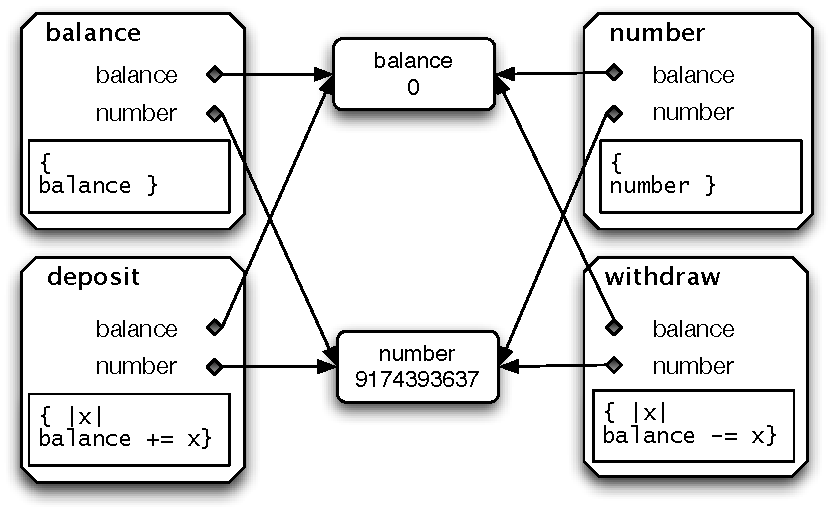
\includegraphics{omnifigs/bank_account_dia}
	}
	\caption{Structure of Bank Account closures}
	\label{fig:bank_account}
\end{figure}

\subsection{Compiled Closures}\label{concepts:compiled_closures}
The TEM is intended to provide trusted execution at commodity prices.
Therefore, the design will be implemented in embedded chips, where persistent
variables are expensive\footnote{Variables' values may change, therefore they would have to be
stored in EEPROM. EEPROM is the slowest and most expensive type of on-chip
memory.}. The following optimization, inspired from \cite{Ste:78b} helps
reduce the amount of shared memory cells used by a closure. Some of the
variable bindings are de-facto immutable (constant). That is, the values of the
bindings will never be modified throughout the lifetime of a closure. This
means that, instead of storing the binding's value in a shared memory location,
the constant value can be stored directly in each closure's binding table. This
eliminates most uses of shared memory locations. \cite{Ste:78b} uses this
mechanism to decide whether frames will be allocated on the stack or in the
heap.

For example, knowing that all the languages used in this section (Scheme, Ruby,
Java) pass primitive types by value (as opposed to passing by reference) allows
us to assert that \texttt{term} in listings \ref{simple_closure:scheme},
\ref{simple_closure:java}, and \ref{simple_closure:ruby} are de-facto
immutable. The proof is quick and straight-forward: \texttt{term} is a
function parameter, therefore it is local to the \texttt{adder} function.
\texttt{fact} is not on the left-hand side of any assignment in \texttt{adder},
therefore it is de-facto immutable.

By a similar argument, it is easy to prove that \texttt{number} in listing
\ref{fig:bank_account} is de-facto immutable, and \texttt{balance} isn't. So
the closures' binding tables can be optimized to use one shared memory location
instead of two, as illustrated in figure \ref{fig:bank_account}.

\begin{figure}[hbtp]
	\center{
		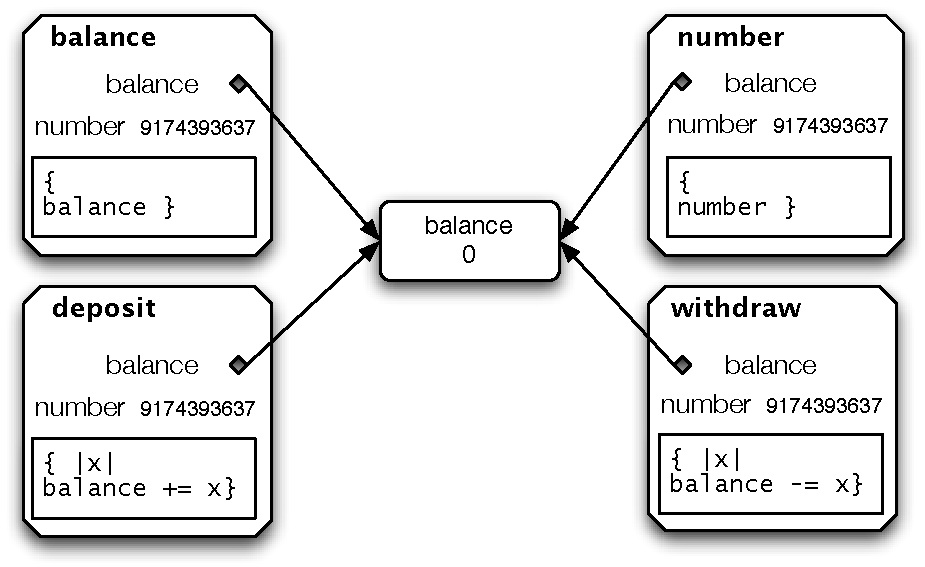
\includegraphics{omnifigs/bank_account_diax}
	}
	\caption{Optimized structure of Bank Account closures}
	\label{fig:bank_account:optimized}
\end{figure}

The result in figure \ref{fig:bank_account:optimized} is further amenable to well-known
optimizations, such as removing the unreferenced entries in the closures'
binding tables. For instance, the variable \texttt{number} is not used at all
in the closures \texttt{balance}, \texttt{deposit}, and \texttt{withdraw}, so
it can be removed from their binding tables.

A \textbf{compiled closure} is a closure that has been fully optimized for the
computer that is intended to execute it. A compiled closure consists of the
following:
\begin{itemize}
  \item the computation to be performed, expressed as executable instructions
  that can be interpreted by the target computer,
  \item a binding table that contains all the non-local variables,
  \item values for the non-local variables that are de-facto immutable, and
  \item addresses (references to shared memory locations) for mutable
  non-local variables.
\end{itemize}

As a note, the approach used in Erlang \cite{carlsson2004cel} deserves interest.
The language has no mutable state, so closures do not need shared memory
locations. This is essential for concurrent programming. Upon further
inspection, I decided that the ideas used to implement mutable state in
Erlang (e.g., Mnesia \cite{mattsson1999mdr}) would prove less efficient than
allowing shared memory cells and using the optimizations described above.

